
\chapter{実験方法}

\section{データセットの作成}
\subsection{撮影環境}
データセットを作成するためにFig.\ref{fig_camera}の環境を構築した.
\begin{figure}[]
  \begin{center}
    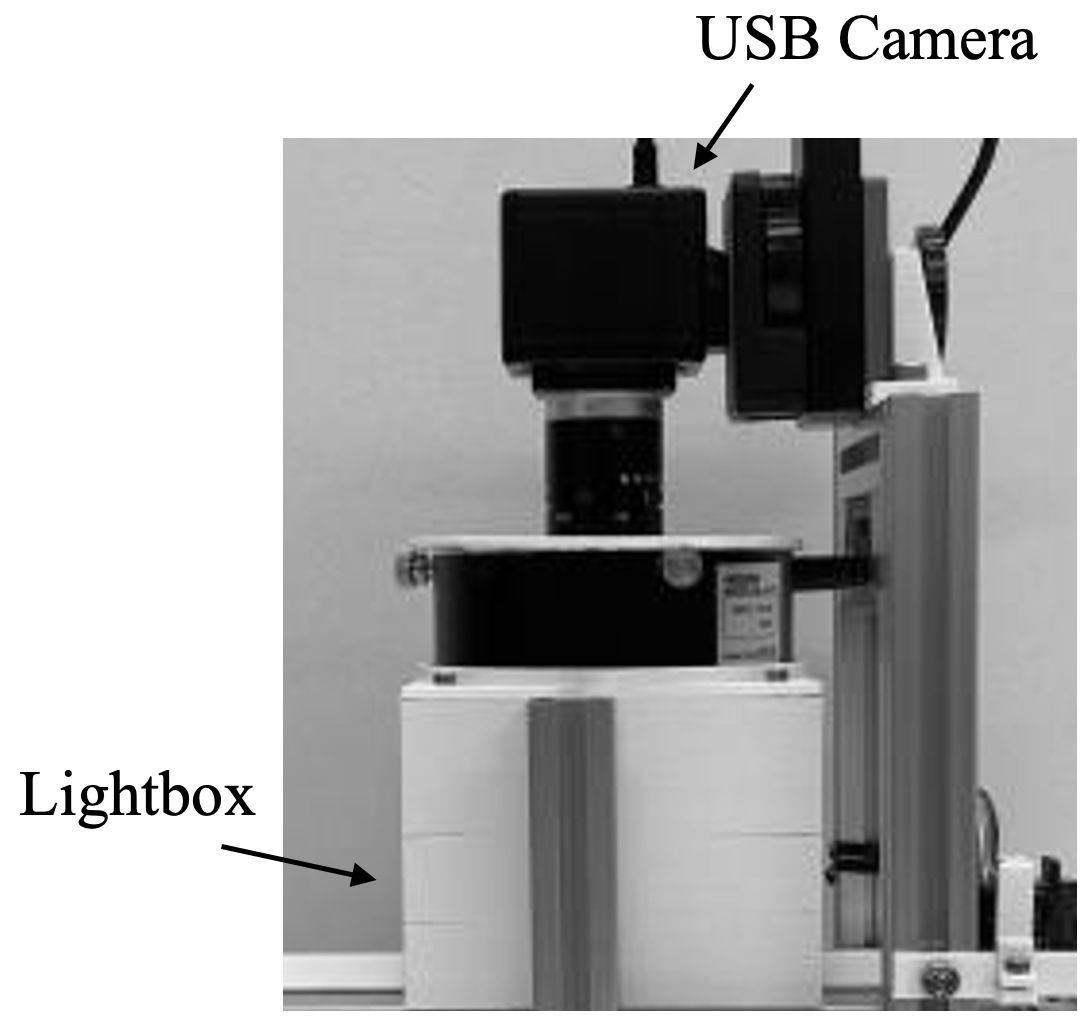
\includegraphics[scale = 0.5]{./chapter3/device.png}
    \caption{撮影環境}
    \label{fig_camera}
  \end{center}
\end{figure}

画像の明度が変わったり影ができてしまうと誤判定の原因となってしまうため,Webカメラに自作のライトボックスを取り付けそれらを起こさないための工夫を施した.なお,本実験で使用したコーヒー豆はコロンビアスプレモとブラジルサントスNo.2の生豆である.

\subsection{画像の前処理}
取得画像には以下の前処理を施した.
\begin{enumerate}
\item ノイズ対策としてメディアンフィルタを用いたぼかし処理.
\item OpenCVを用いて画像をグレースケール化し2値化をする.コーヒー豆部分が黒く,背景が白い画像を生成.
\item 2値化した画像を反転し,コーヒー豆内のノイズを塗りつぶす.コーヒー豆部分が白く,背景が黒い画像を生成.
\item その画像を元の画像と掛け合わせ,マスキングを行う.元の画像の背景のみ黒く塗りつぶす.
\item コーヒー豆の重心を求め,$100\times 100$ピクセルに切り出す
\item コーヒー豆を縦向きに補正
\item 画像を$80\times 80$にリサイズし,コントラストを上げる.
\end{enumerate}

データセットの構成は以下の通りである.なお,これらをデータセットとしてネットワークへ入力した上で学習時に都度左右反転,上下反転,左右上下反転,回転を加えデータセットの拡張を行っている.
\begin{itemize}
  \item 学習データ:3981枚
  \item テストデータ:789枚
\end{itemize}

\section{ネットワークの構造}
本実験のネットワークの構造を図\ref{fig_nnst}に示す.
\begin{figure}[]
  \begin{center}
    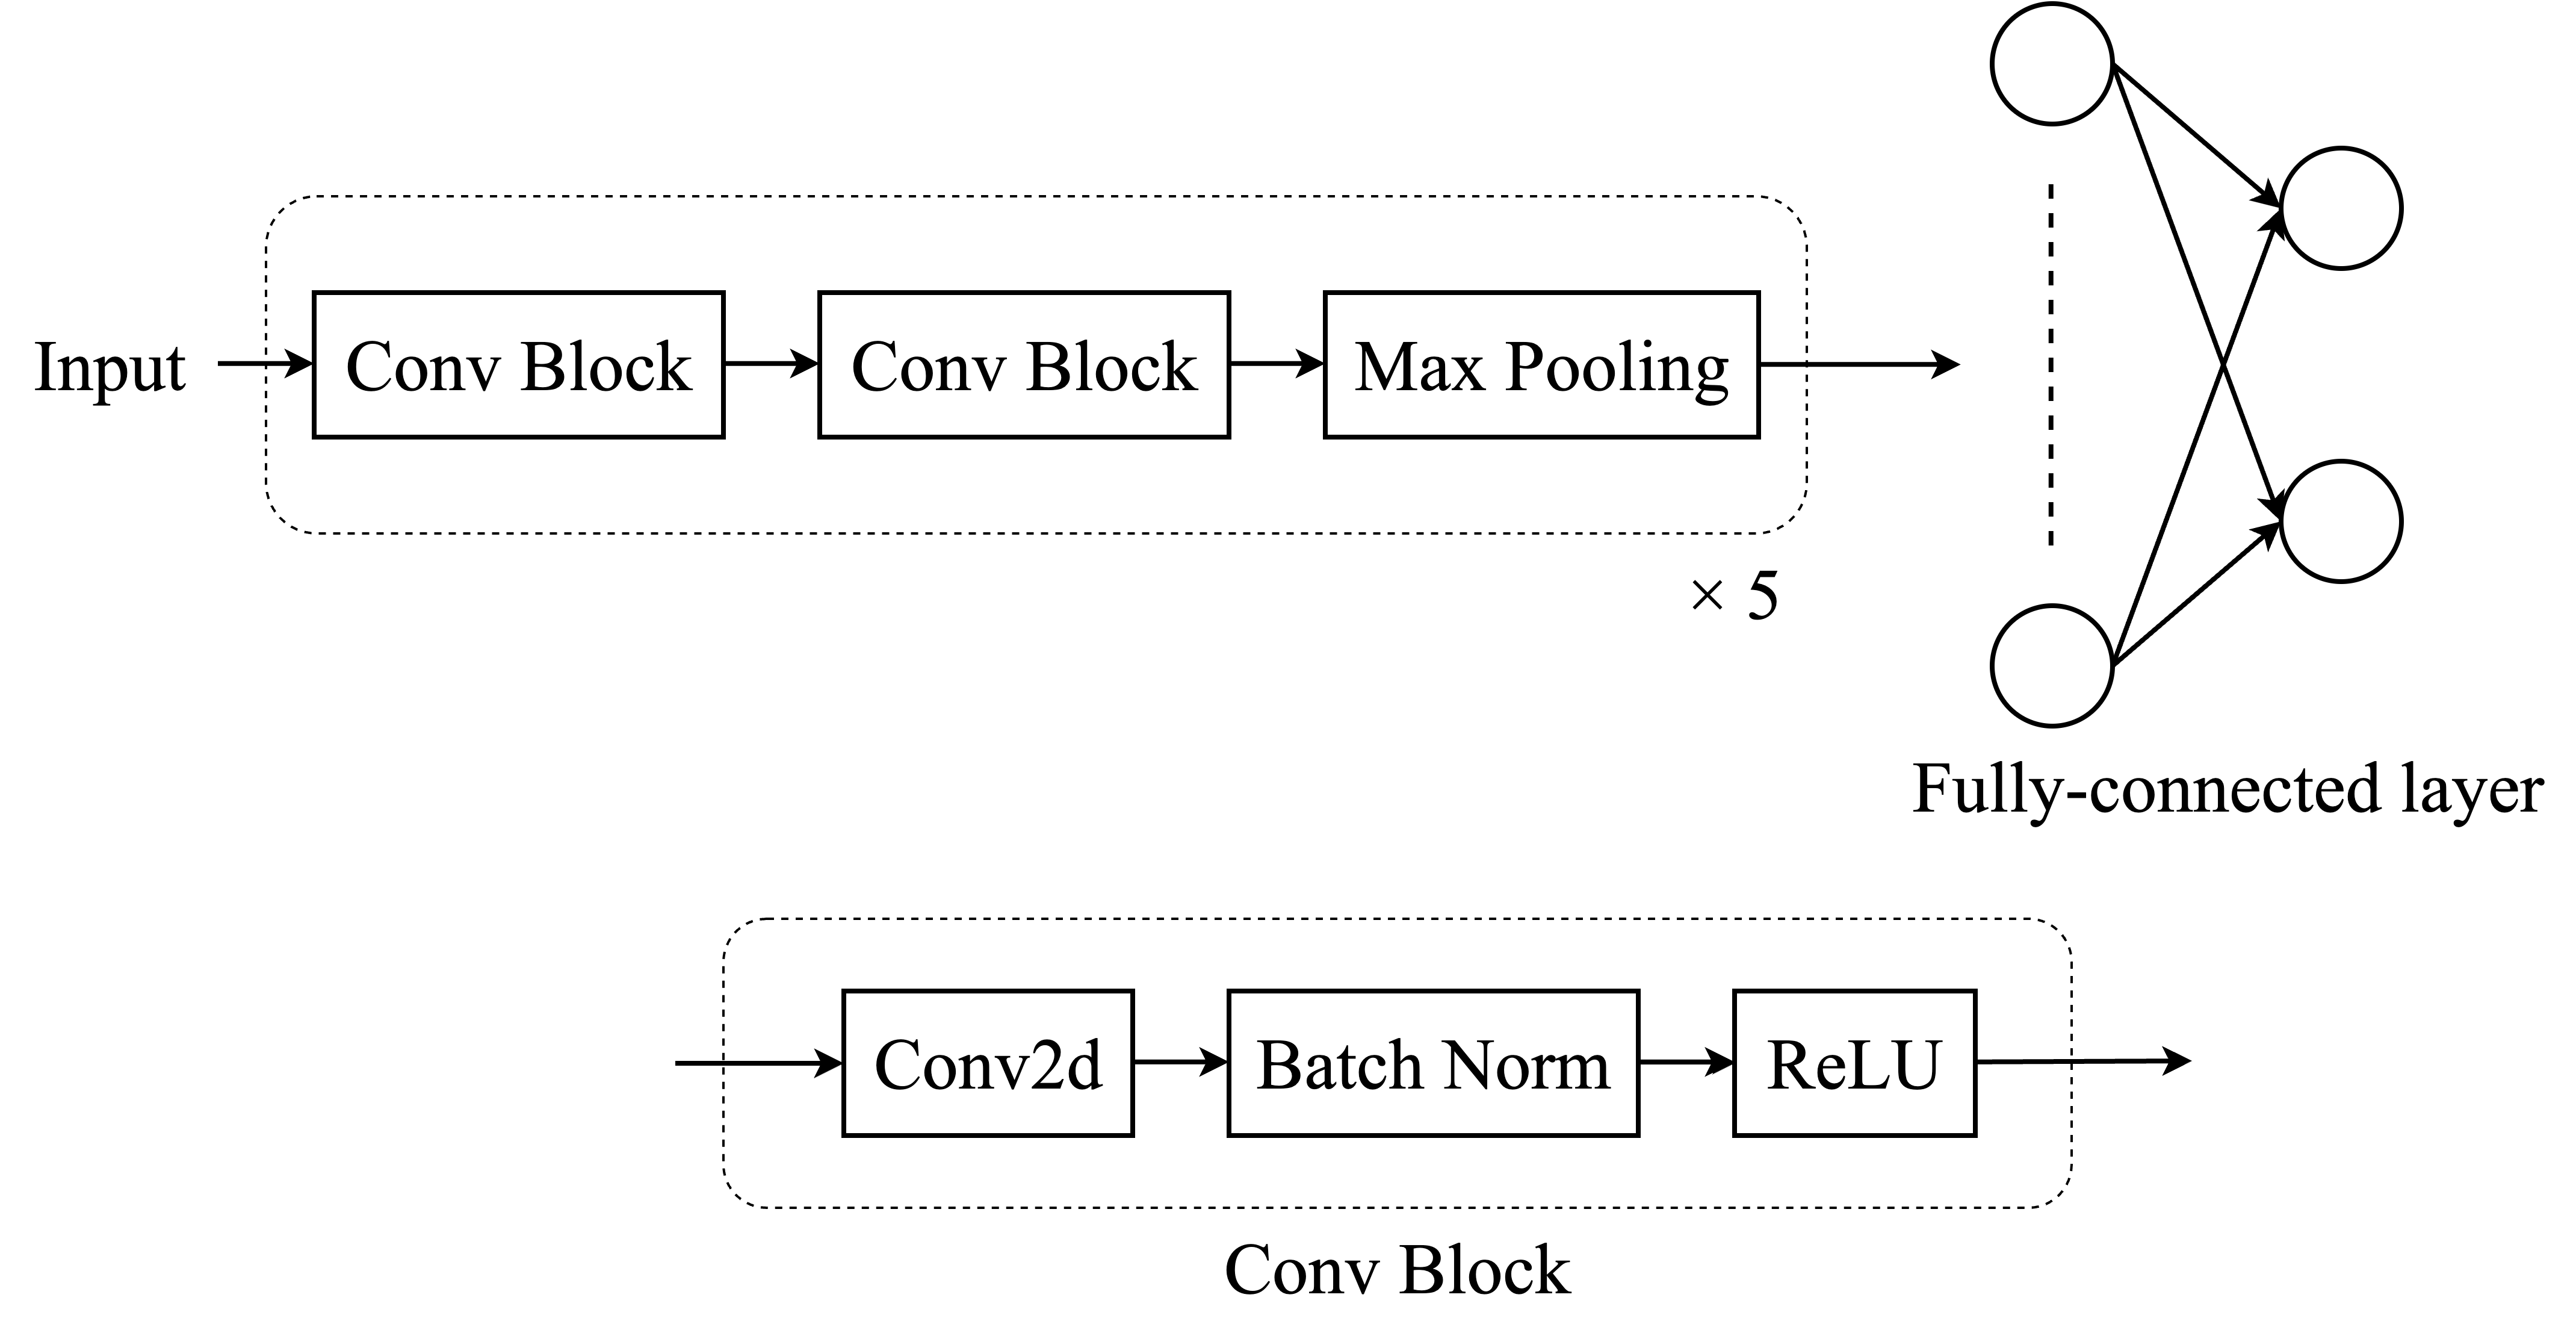
\includegraphics[scale = 0.06]{./chapter3/nn_struct.png}
    \caption{ネットワークの構造}
    \label{fig_nnst}
  \end{center}
\end{figure}

畳み込み,Batch Normalization,ReLUを1セットとした時それを5回繰り返すため畳み込み層は合計で10層である.また,畳み込み層2層ごとにMax Poolingを行っている.そして,畳み込み層での結果を全結合層へ渡し,全結合層の出力は良否の2パターンになっている.ここで,10層の畳み込み層を$C_i = C_1 \ldots C_{10}$とし,各層のパラメータは表.\ref{table_network_parameter}にまとめる.
\begin{table}
  \caption{ネットワークのパラメータ}
  \label{table_network_parameter}
  \centering
  \begin{tabular}{ccc}
    \hline
    畳み込み層  & カーネルサイズ & 出力ch \\
    \hline \hline
    $C_1$,$C_2$ & $3\times 3$ & 16\\
    $C_3$,$C_4$ & $3\times 3$ & 32\\
    $C_5$,$C_6$ & $3\times 3$ & 64\\
    $C_7$,$C_8$ & $3\times 3$ & 128\\
    $C_9$,$C_10$ & $3\times 3$ & 256\\
    \hline
    Max Pooling & カーネルサイズ$2\times 2$ & ストライド2\\
    全結合層 & 入力256 & 出力2\\
    \hline
  \end{tabular}
\end{table}

畳み込み層はPadding size1で0Paddingを行っておりMax Poolingでのみ画像サイズが変わっている.